%%%% Paramétrage du TD %%%%

\def\xxnumchapitre{Chapitre 2 \vspace{.2cm}}
\def\xxchapitre{\hspace{.12cm} Révisions SLCI}

\def\xxcompetences{%
\textsl{%
\textbf{Savoirs et compétences :}\\
\vspace{-.4cm}
\begin{itemize}[label=\ding{112},font=\color{bleuxp}] 
\item .
%\item \textit{Mod3.C2 : } pôles dominants et réduction de l’ordre du modèle : principe, justification
\end{itemize}
}}

\def\xxfigures{
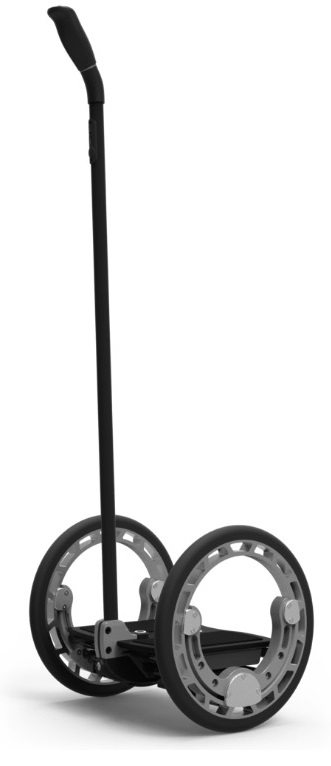
\includegraphics[width=.6\textwidth]{fig_01}
%\textit{}
}%figues de la page de garde
\def\xxtitreexo{Système de freinage d’un TGV DUPLEX}
\def\xxsourceexo{\hspace{.2cm} \footnotesize{Concours Centrale Supelec PSI 2006} \ifprof-- Ressources UPSTI\else\fi}

\def\xxactivite{{Synthèse 03} \ifprof  -- Corrigé \else \fi}

%\iflivret
\input{\repRel/Style/pagegarde_TD}
%\else
%\pagestyle{empty}


%%%%%%%% PAGE DE GARDE COURS
\ifcours
\begin{tikzpicture}[remember picture,overlay]
\node at (current page.north west)
{\begin{tikzpicture}[remember picture,overlay]
\node[anchor=north west,inner sep=0pt] at (0,0) {\includegraphics[width=\paperwidth]{\thechapterimage}};
\draw[anchor=west] (-2cm,-8cm) node [line width=2pt,rounded corners=15pt,draw=ocre,fill=white,fill opacity=0.6,inner sep=40pt]{\strut\makebox[22cm]{}};
\draw[anchor=west] (1cm,-8cm) node {\huge\sffamily\bfseries\color{black} %
\begin{minipage}{1cm}
\rotatebox{90}{\LARGE\sffamily\textsc{\color{ocre}\textbf{\xxnumpartie}}}
\end{minipage} \hfill
\begin{minipage}[c]{14cm}
\begin{titrepartie}
\begin{flushright}
\renewcommand{\baselinestretch}{1.1} 
\Large\sffamily\textsc{\textbf{\xxpartie}}
\renewcommand{\baselinestretch}{1} 
\end{flushright}
\end{titrepartie}
\end{minipage} \hfill
\begin{minipage}[c]{3.5cm}
{\large\sffamily\textsc{\textbf{\color{ocre} \discipline}}}
\end{minipage} 
 };
\end{tikzpicture}};
\end{tikzpicture}


\begin{tikzpicture}[overlay]
\node[shape=rectangle, 
      rounded corners = .25 cm,
	  draw= ocre,
	  line width=2pt, 
	  fill = ocre!10,
	  minimum width  = 2.5cm,
	  minimum height = 3cm,] at (18cm,0) {};
\node at (17.7cm,0) {\rotatebox{90}{\textbf{\Large\color{ocre}{\classe}}}};
%{};
\end{tikzpicture}

\vspace{3.5cm}

\begin{tikzpicture}[remember picture,overlay]
\draw[anchor=west] (-2cm,-6cm) node {\huge\sffamily\bfseries\color{black} %
\begin{minipage}{2cm}
\begin{center}
\LARGE\sffamily\textsc{\color{ocre}\textbf{\xxactivite}}
\end{center}
\end{minipage} \hfill
\begin{minipage}[c]{15cm}
\begin{titrechapitre}
\renewcommand{\baselinestretch}{1.1} 
\Large\sffamily\textsc{\textbf{\xxnumchapitre}}

\Large\sffamily\textsc{\textbf{\xxchapitre}}
\vspace{.5cm}

\renewcommand{\baselinestretch}{1} 
\normalsize\normalfont
\xxcompetences
\end{titrechapitre}
\end{minipage}  };
\end{tikzpicture}
\vfill

\begin{flushright}
\begin{minipage}[c]{.3\linewidth}
\begin{center}
\xxfigures
\end{center}
\end{minipage}\hfill
\begin{minipage}[c]{.6\linewidth}
\startcontents
\printcontents{}{1}{}
\end{minipage}
\end{flushright}

\begin{tikzpicture}[remember picture,overlay]
\draw[anchor=west] (4.5cm,-.7cm) node {
\begin{minipage}[c]{.2\linewidth}
\begin{flushright}

\includegraphics[width=2cm]{png/logoCC}
\end{flushright}
\end{minipage}
\begin{minipage}[c]{.2\linewidth}
\textsl{\xxauteur} \\
\textsl{\classe}
\end{minipage}
 };
\end{tikzpicture}
\newpage
\pagestyle{fancy}

\newpage
\pagestyle{fancy}

\else
\fi


%%%%%%%% PAGE DE GARDE TD
\iftd
%\begin{tikzpicture}[remember picture,overlay]
%\node at (current page.north west)
%{\begin{tikzpicture}[remember picture,overlay]
%\draw[anchor=west] (-2cm,-3.25cm) node [line width=2pt,rounded corners=15pt,draw=ocre,fill=white,fill opacity=0.6,inner sep=40pt]{\strut\makebox[22cm]{}};
%\draw[anchor=west] (1cm,-3.25cm) node {\huge\sffamily\bfseries\color{black} %
%\begin{minipage}{1cm}
%\rotatebox{90}{\LARGE\sffamily\textsc{\color{ocre}\textbf{\xxnumpartie}}}
%\end{minipage} \hfill
%\begin{minipage}[c]{13.5cm}
%\begin{titrepartie}
%\begin{flushright}
%\renewcommand{\baselinestretch}{1.1} 
%\Large\sffamily\textsc{\textbf{\xxpartie}}
%\renewcommand{\baselinestretch}{1} 
%\end{flushright}
%\end{titrepartie}
%\end{minipage} \hfill
%\begin{minipage}[c]{3.5cm}
%{\large\sffamily\textsc{\textbf{\color{ocre} \discipline}}}
%\end{minipage} 
% };
%\end{tikzpicture}};
%\end{tikzpicture}

%%%%%%%%%% PAGE DE GARDE TD %%%%%%%%%%%%%%%
%\begin{tikzpicture}[overlay]
%\node[shape=rectangle, 
%      rounded corners = .25 cm,
%	  draw= ocre,
%	  line width=2pt, 
%	  fill = ocre!10,
%	  minimum width  = 2.5cm,
%	  minimum height = 2.5cm,] at (18.5cm,0) {};
%\node at (17.7cm,0) {\rotatebox{90}{\textbf{\Large\color{ocre}{\classe}}}};
%%{};
%\end{tikzpicture}

% PARTIE ET CHAPITRE
%\begin{tikzpicture}[remember picture,overlay]
%\draw[anchor=west] (-1cm,-2.1cm) node {\large\sffamily\bfseries\color{black} %
%\begin{minipage}[c]{15cm}
%\begin{flushleft}
%\xxnumchapitre \\
%\xxchapitre
%\end{flushleft}
%\end{minipage}  };
%\end{tikzpicture}

% Bandeau titre exo
\begin{tikzpicture}[remember picture,overlay]
\draw[anchor=west] (-2cm,-6cm) node {\huge\sffamily\bfseries\color{black} %
\begin{minipage}{5cm}
\begin{center}
\LARGE\sffamily\color{ocre}\textbf{\textsc{\xxactivite}}

\begin{center}
\xxfigures
\end{center}

\end{center}
\end{minipage} \hfill
\begin{minipage}[c]{12cm}
\begin{titrechapitre}
\renewcommand{\baselinestretch}{1.1} 
\large\sffamily\textbf{\textsc{\xxtitreexo}}

\small\sffamily{\textbf{\textit{\color{black!70}\xxsourceexo}}}
\vspace{.5cm}

\renewcommand{\baselinestretch}{1} 
\normalsize\normalfont
\xxcompetences
\end{titrechapitre}
\end{minipage}  };
\end{tikzpicture}

\else
\fi


%%%%%%%% PAGE DE GARDE FICHE
\iffiche
\begin{tikzpicture}[remember picture,overlay]
\node at (current page.north west)
{\begin{tikzpicture}[remember picture,overlay]
\draw[anchor=west] (-2cm,-3.25cm) node [line width=2pt,rounded corners=15pt,draw=ocre,fill=white,fill opacity=0.6,inner sep=40pt]{\strut\makebox[22cm]{}};
\draw[anchor=west] (1cm,-3.25cm) node {\huge\sffamily\bfseries\color{black} %
\begin{minipage}{1cm}
\rotatebox{90}{\LARGE\sffamily\textsc{\color{ocre}\textbf{\xxnumpartie}}}
\end{minipage} \hfill
\begin{minipage}[c]{14cm}
\begin{titrepartie}
\begin{flushright}
\renewcommand{\baselinestretch}{1.1} 
\large\sffamily\textsc{\textbf{\xxpartie} \\} 

\vspace{.2cm}

\normalsize\sffamily\textsc{\textbf{\xxnumchapitre -- \xxchapitre}}
\renewcommand{\baselinestretch}{1} 
\end{flushright}
\end{titrepartie}
\end{minipage} \hfill
\begin{minipage}[c]{3.5cm}
{\large\sffamily\textsc{\textbf{\color{ocre} \discipline}}}
\end{minipage} 
 };
\end{tikzpicture}};
\end{tikzpicture}


\begin{tikzpicture}[overlay]
\node[shape=rectangle, 
      rounded corners = .25 cm,
	  draw= ocre,
	  line width=2pt, 
	  fill = ocre!10,
	  minimum width  = 2.5cm,
%	  minimum height = 2.5cm,] at (18.5cm,0.5cm) {};
	  minimum height = 2.5cm,] at (18.5cm,0cm) {};
\node at (17.7cm,0) {\rotatebox{90}{\textsf{\textbf{\large\color{ocre}{\classe}}}}};
%{};
\end{tikzpicture}



\else
\fi



%\fi

\setlength{\columnseprule}{.1pt}

\pagestyle{fancy}
\thispagestyle{plain}

\vspace{4.5cm}

\def\columnseprulecolor{\color{bleuxp}}
\setlength{\columnseprule}{0.4pt} 
\setcounter{numques}{0}
%%%%%%%%%%%%%%%%%%%%%%%

\ifprof
\else
\begin{multicols}{2}
\fi

\section*{Mise en situation}

\ifprof
\else
L’objet de cette étude est l’analyse du système de freinage mécanique à énergie
pneumatique installé sur les TGV Duplex. Par soucis de sécurité, il est indispensable d'éviter le blocage des roues (phénomène appelé enrayage) lors du freinage. Pour cela il est nécessaire de maîtriser la vitesse de glissement entre la roue et le rail.
\begin{obj}
L’objectif est d'étudier la loi de commande du dispositif d’anti-enrayage et plus précisément le calcul du correcteur de la boucle de régulation.
\end{obj}


%La réalisation de la régulation de glissement entre la roue et le rail ne peut être effectuée directement, en particulier la seule mesure généralement disponible est celle de la vitesse, aussi la vitesse est obtenue par estimation. 


%En « pratique », la mise en place de la chaîne de régulation du dispositif d’anti-enrayage du système de freinage est conçue de la façon suivante :
%\begin{itemize}
%\item elle est réalisée au travers de l’asservissement des vitesses des roues à une
%consigne de référence obtenue à partir de $V_T$ (vitesse de translation du train par rapport aux rails);
%\item la commande de l’actionneur est non linéaire, de type tout ou rien ;
%\item les algorithmes implémentés visent à optimiser le point de fonctionnement
%en vue de minimiser la distance de freinage.
%Cependant, dans le cadre de cette étude, on supposera que :
%\item les vitesses $V_R$ (l’opposée de la vitesse du point de contact appartenant à la roue par
%rapport au bogie) et $V_T$ sont directement accessibles à la mesure, éventuellement
%entachées d’une erreur ;
%\item la régulation peut se ramener directement à celle du glissement ;
%\item le comportement de l’actionneur et de sa « commande rapprochée » est modélisé
%par une fonction de transfert linéaire correspondant à un comportement « moyen ».
%\end{itemize}

On suppose, pour la suite, que l’architecture de la boucle de régulation est représentée sur la figure suivante où $\nu_c$ est la consigne de glissement.

\begin{center}
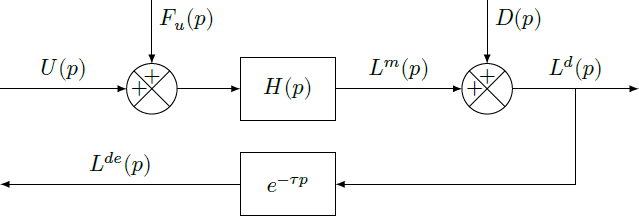
\includegraphics[width=\linewidth]{fig_02}
\textit{Structure de la chaîne de régulation de glissement}
\end{center}

On note : 
\begin{itemize}
\item $H_1(p)$ la fonction de transfert de l’actionneur de freinage (vérin pneumatique + électrovalve) ;
\item $H_2(p)$ la fonction de transfert de la roue au freinage;
\item $C(p)$ le correcteur de la boucle de régulation ;
\item $M(p)$ la fonction de transfert de la chaîne de mesure du glissement,% obtenu à partir des vitesses $V_T$ et $V_R$
 cette chaîne comporte un filtre destiné à limiter l’impact des bruits de mesure;
\item $\nu_m$ : glissement estimé.% à partir de $V_T$ et de $V_R$.
\end{itemize}
On adoptera pour la suite : $H_1(p)=\dfrac{2000}{1+0,1p+0,01p^2}$ et $M(p)=\dfrac{1}{1+0,05p}$.

Pour une vitesse de train $V_T=\SI{200}{km.h^{-1}}$, le cahier des charges est résumé par les données du tableau suivant et les données numériques utilisées sont données ci-dessous.
Enfin, les problèmes liés à l’évolution de la vitesse du train par rapport au rail $V_T$ ne font pas l’objet de cette étude.

On a $M=\SI{8200}{kg}$, $V_T=\SI{200}{km.h^{-1}}$, $I/r^2=\SI{400}{kg}$, $g=\SI{10}{m.s^{-2}}$.

\footnotesize
\begin{center}
\begin{tabular}{|p{.6\linewidth}|p{.3\linewidth}|}
\hline
\multicolumn{2}{|l|}{\textbf{Marges de stabilité, performances en boucle ouverte}} \\ \hline
Pulsation de coupure à \SI{0}{dB} & $\omega_c \simeq \SI{1}{rad.s^{-1}}$ \\ \hline
Marge de phase & $\Delta \varphi \geq 60\degres$ au point de fonctionnement nominal $B$ \\ \hline
Stabilité quel que soit le point de fonctionnement sur la caractéristique $\mu = f(\nu)$ & \\ \hline
\multicolumn{2}{|l|}{\textbf{Réponse à un échelon de consigne de glissement}} \\ \hline
Écart en régime permanent & Nul \\ \hline
Temps du 1\ier maximum & $t_m\leq \SI{3,5}{s}$ \\ \hline
Dépassement & $D\simeq  18\, \%$  \\ \hline
\multicolumn{2}{|l|}{\textbf{Réponse à une variation en échelon de l'adhérence}} \\ \hline
Écart en régime permanent & Nul \\ \hline
Temps de réponse & $t_r \leq \SI{9}{s}$ \\
\hline
\end{tabular}
\end{center}

\normalsize

\begin{center}
%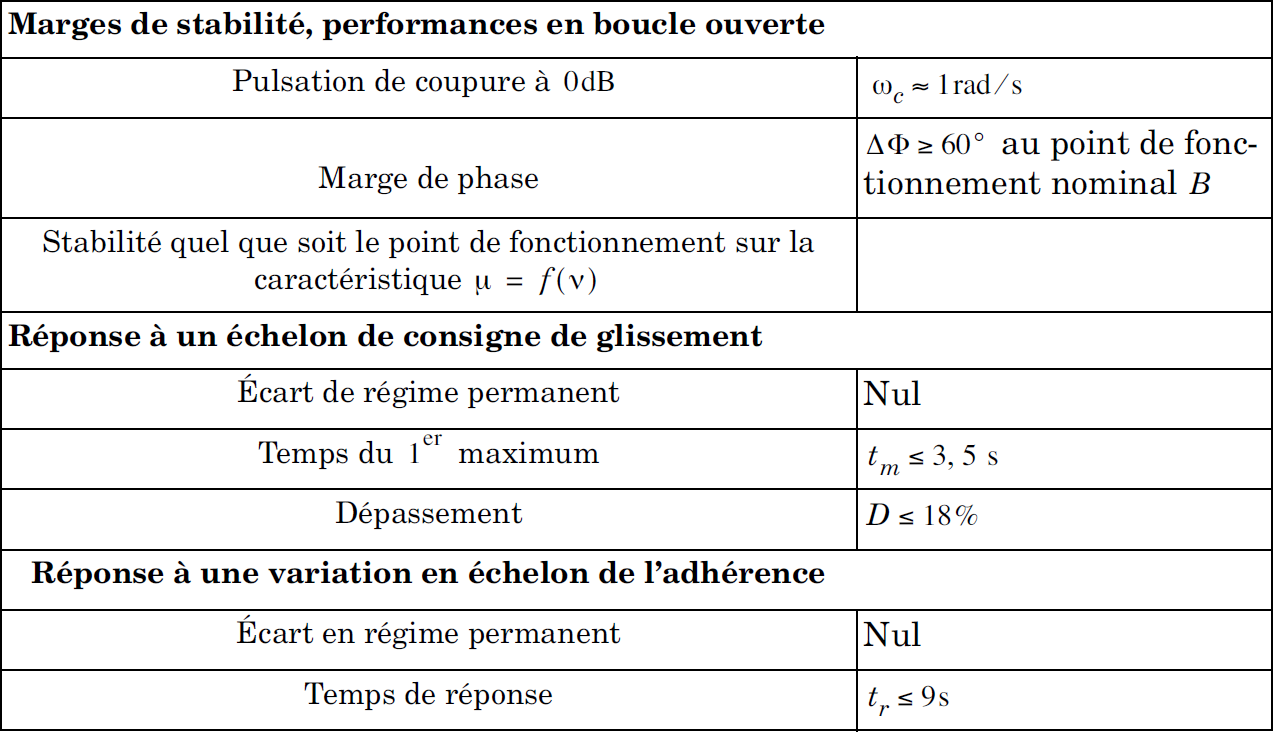
\includegraphics[width=\linewidth]{fig_02a}
\textit{Cahier des charges de la boucle de régulation de glissement pour $V_T = \SI{200}{km.h^{-1}}$}
\end{center}
\fi


\subsection*{Analyse des réponses fréquentielles en boucle ouverte}
\ifprof
\else
On donne la fonction de transfert entre le glissement relatif et la force de freinage : $H_2(p)=\dfrac{\nu_1 (p)}{F_R(p)}=\dfrac{45\cdot 10^{-6}}{p}$.

\fi
%\dfrac{1}{gMf'\left(\nu_0\right)} \dfrac{1}{1+\dfrac{IV_{T0}}{r^2g Mf'\left(\nu_0\right)}p} = \dfrac{K}{1+\tau p}.
%$$

%\question{En utilisant la relation précédente, préciser la fonction de transfert $H_2(p)$ autour du point de fonctionnement sous forme numérique.}
%\ifprof
%\begin{corrige}
%\end{corrige}
%\else
%\fi


\question{En prenant $C(p)=1$, compléter par le tracé asymptotique le diagramme
de Bode de la fonction de transfert en boucle ouverte fourni.}% en annexe 3
%en justifiant le tracé sur la copie (document réponse à joindre obligatoirement
%avec la copie). Pour la suite, vous pourrez adopter sans aucune justification le
%diagramme de Bode de l’annexe 3.}

\ifprof
\else
\begin{center}
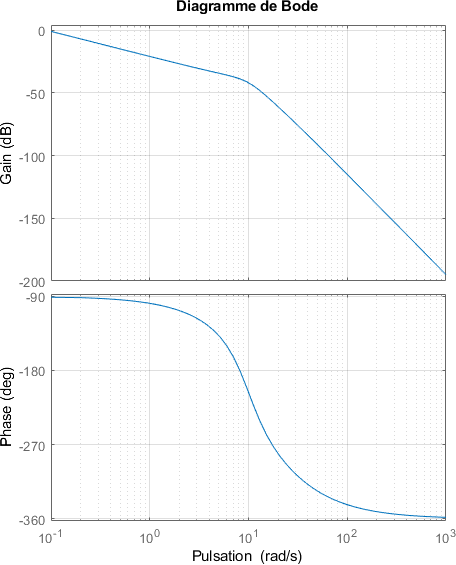
\includegraphics[width=\linewidth]{BodeQ1}
%\textit{Cahier des charges de la boucle de régulation de glissement pour $V_T = \SI{200}{km.h^{-1}}$}
\end{center}
\fi

\ifprof
\begin{corrige}
On a pour $H_1(p)$, $\dfrac{1}{\omega_0^2}=0,01 \Leftrightarrow \omega_0=10$ et $2\dfrac{\xi}{\omega_0}=0,1$ soit $\xi = 0,1\times 10 / 2 = 0,5$. Les pulsations caractéristiques de la FTBO sont donc $\omega_0=\SI{10}{rad.s^{-1}}$ et $1/0,05 = \SI{20}{rad.s^{-1}}$.

Pour tracer un diagramme de Bode avec un intégrateur, il est nécessaire de définir un point pour définir la << hauteur >> du tracé. Pour cela on prend un point pour lequel seul l'intégrateur et les constantes ont de l'effet. Ainsi, pour $\omega=\SI{0,1}{rad.s^{-1}}$, on a $\text{FTBO}(p) \simeq \dfrac{2000\times 45\times 10^{-6}}{p}$. On a donc $20\log 0,09 - 20 \log 0,1 \simeq \SI{-0,92}{dB}$.

On peut dresser le tableau de variations de la FTBO puis tracer les asymptotes. 
\begin{center}
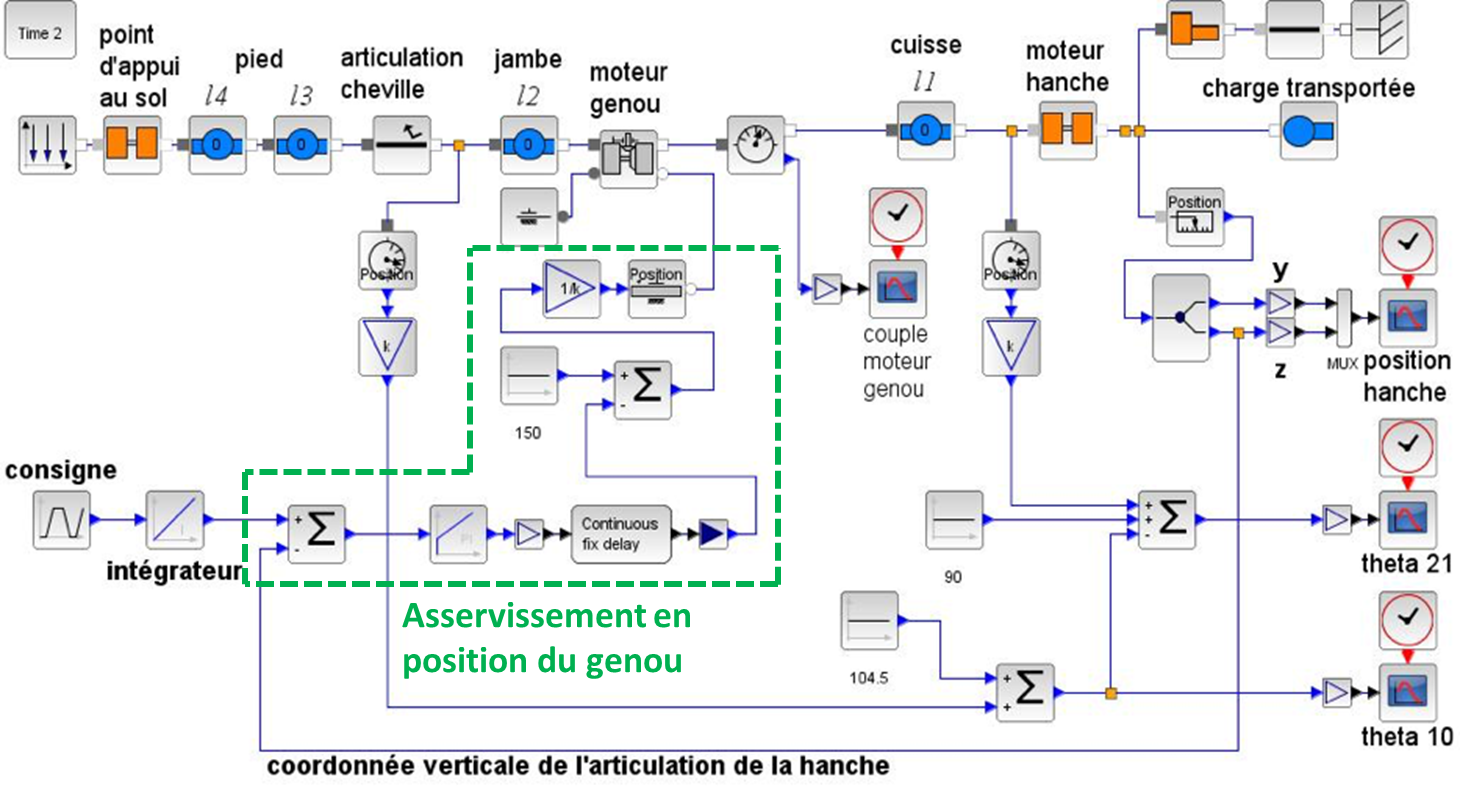
\includegraphics[width=\linewidth]{cor_01}
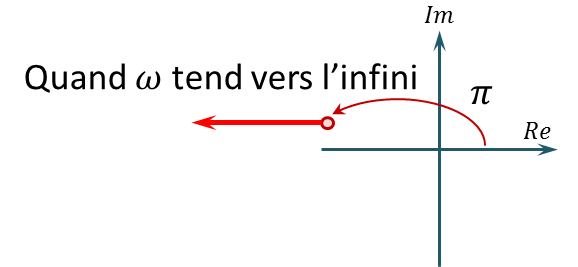
\includegraphics[width=\linewidth]{cor_02}
\end{center}
\end{corrige}
\else
\fi

\subsection*{Synthèse du régulateur de la boucle de régulation}

On décide d’implémenter un régulateur de type P.I. dont la fonction de transfert
est : $C(p)=K_r\left(1+\dfrac{1}{T_i p} \right)$.

\question{Calculer la valeur que doit prendre l’argument de $C(p)$ afin d’assurer
la marge de phase imposée par le cahier des charges à la pulsation de coupure $\omega_c$
souhaitée.}

\footnotesize
\begin{methode}
Si on note $\omega_c$ on définit la pulsation de coupure telle que $|\text{FTBO}\left(j \omega_c \right)| = \SI{0}{dB}$. On peut alors définir la marge de phase par $M\varphi=\arg \left[\text{FTBO}\left( j \omega_c\right)\right]-\left(-180\degres\right)$.
\end{methode}

\normalsize 

\ifprof
\begin{corrige}
La pulsation de coupure souhaitée est $\omega_c \simeq \SI{1}{rad.s^{-1}}$. 
On cherche donc $K_r$ et $T_i$ tels que $\arg \left[\text{FTBO}\left( j \omega_c\right)\right]-\left(-180\degres\right)=60\degres$.

$\arg \left[\text{FTBO}\left( j \omega\right)\right]$ 
$ = \arg \left[
\underbrace{\dfrac{2000}{1+0,1p+0,01p^2}}_{\to \SI{-5,7}{\degres} \text{ qd } \omega=\omega_c} 
\cdot
\underbrace{\dfrac{1}{1+0,05p}}_{\to \SI{-2,8}{\degres} \text{ qd } \omega=\omega_c} 
\cdot 
 \underbrace{K_r}_{\to 0}
 \left(1+\dfrac{1}{T_i p} \right) \cdot 
\underbrace{\dfrac{45\cdot 10^{-6}}{p}}_{\to -90\degres } 
\right] $
$ = \arg \left[  \left(1+\dfrac{1}{T_i p} \right) \right] -98,5$

\begin{rem}
Ci-dessus, ce sont les \textbf{arguments} que l'on évalue lorsque $\omega=\omega_c$. L'argument du produit est égal à la somme des arguments.
\end{rem}
$ \arg \left[\text{FTBO}\left( j \omega\right)\right] = \arg \left[  \dfrac{T_i p+1}{T_i p}  \right]-98,5 $.
%$ = \arctan (T_i \omega) -98,5-90$.

Pour respecter la marge souhaitée, il est donc nécessaire que 
$\arg \left[\text{FTBO}\left( j \omega_c\right)\right]-\left(-180\right)\geq60$
Soit 
$\arg \left[  \dfrac{T_i p+1}{T_i p}  \right]-98,5+ 180 \geq60$ 
et $\arg \left[  \dfrac{T_i p+1}{T_i p}  \right] \geq - \SI{21,5}{\degres}$.
 
\end{corrige}
\else
\fi

\question{Calculer la valeur minimale, $T_{\text{imin}}$, que l’on peut conférer à la constante $T_i$ de l’action intégrale du régulateur.}

\ifprof
\begin{corrige}
On en déduit que pour $\omega=\omega_c=1$, 
$\arg \left[  \dfrac{T_i p+1}{T_i p}  \right] \geq - \SI{21,5}{\degres}$
$ \Leftrightarrow  \arctan (T_i \omega) -90 \geq - \SI{21,5}{\degres}$ 
$ \Leftrightarrow  \arctan (T_i \omega)  \geq \SI{68,5}{\degres}$ 
et donc $\Rightarrow  T_i \geq \tan(68,5)=\SI{2,54}{s}$.
 

 \begin{warn}
\textbf{Attention} : à ce stade, la marge de phase serait de 60\degres \textbf{SI} la pulsation de  coupure était de \SI{1}{rad.s^{-1}} ce qui n'est pas encore le cas pour le moemnt.
 \end{warn}
 
\end{corrige}
\else
\fi


\question{En adoptant $T_{i}=T_{\text{imin}}$, déterminer alors le gain $K_r$ du régulateur permettant de satisfaire la pulsation de coupure et la marge de phase souhaitées. (Approche graphique demandée, approche analytique facultative)}
%ECRIRE CONDITION

\begin{methode}
Il faut chercher $K_r$ tel que $20\log||\text{FTBO}(j\omega_c)||=0$.
\end{methode}
\ifprof


\ifprof
\begin{corrige}
En raisonnant graphiquement à l'aide du diagramme en boucle ouverte non corrigé, on lit que le gain est d'environ \SI{-20}{dB} lorsque $\omega=1$. La fonction de transfert du correcteur est 
$C(p)=K_r  \left(1+\dfrac{1}{T_i p} \right)=K_r  \dfrac{T_i p+1}{T_i p} $. Le gain dB du correcteur doit donc être de \SI{20}{dB} lorsque $\omega=1$ :
$20\log K_r  +20\log \sqrt{T_i^2 \omega^2 + 1}- 20\log T_i \omega =20$
$\Leftrightarrow \log K_r  +\log \sqrt{T_i^2  + 1}- \log T_i  =1$
$\Leftrightarrow \log K_r   =1-\log \sqrt{T_i^2  + 1}+ \log T_i $. 

On a donc $K_r = 9,3$. 

\vspace{1cm}
Anlaytiquement (à vérifier....)
$20\log||\text{FTBO}(j\omega_c)||=0 \Rightarrow ||\text{FTBO}(j\omega_c)||=1$.

$\left|\left| \text{FTBO}\left( j \omega\right)\right|\right|$ 
$ = \left|\left|
{\dfrac{2000}{1+0,1p+0,01p^2}}
\cdot
{\dfrac{1}{1+0,05p}}
\cdot 
{K_r}
 \left(1+\dfrac{1}{T_i p} \right) \cdot 
\dfrac{45\cdot 10^{-6}}{p}
\right|\right| $

$ = \left|\left|
{\dfrac{2000}{1+0,1p+0,01p^2}}
\cdot
{\dfrac{1}{1+0,05p}}
\cdot 
{K_r}
 \dfrac{1+T_i p}{T_i p} 
\dfrac{45\cdot 10^{-6}}{p}
\right|\right| $

$ =  \dfrac{K_r}{T_i\omega^2}  90\cdot 10^{-3}  \sqrt{1+T_i^2\omega^2}\left|\left|
\dfrac{1}{1+0,1p+0,01p^2}
\dfrac{1}{1+0,05p}
\right|\right| $
$ =  \dfrac{K_r}{T_i\omega^2}  90\cdot 10^{-3}  
\dfrac{\sqrt{1+T_i^2\omega^2}}{\sqrt{1+0,05^2 \omega^2}}
\dfrac{1}{\sqrt{\left(1-0,01^2\omega^2\right)^2+0,1^2\omega^2}} $

$ =  \dfrac{K_r}{T_i}  90\cdot 10^{-3}  
\dfrac{\sqrt{1+T_i^2}}{\sqrt{1+0,05^2 }}
\dfrac{1}{\sqrt{\left(1-0,01^2\right)^2+0,1^2}} $

\end{corrige}
\else
\fi


\question{Le système étant bouclé par le régulateur dimensionné à la question
précédente, déterminer la marge de gain. Conclure sur les marges de stabilité obtenues. (Approche graphique demandée, approche analytique facultative)}
\begin{methode}
Soit $\omega_{\varphi}$ la pulsation telle que $\varphi\left(\omega_{\varphi} \right)=-180\degres$. La marge de gain s'exprime alors par $MG=-20\log||H\left(j \omega_{\varphi} \right)||$.
\end{methode}


\begin{corrige}
\textbf{Approche analytique}
On résout $\arg \left[\text{FTBO}\left( j \omega\right)\right] = -180 \degres$ 


$\arg \left[\text{FTBO}\left( j \omega\right)\right]$ 
$ = \arg \left[
\dfrac{2000}{1+0,1p+0,01p^2}
\cdot
\dfrac{1}{1+0,05p}
\cdot 
K_r
 \left(1+\dfrac{1}{T_i p} \right) \cdot 
\dfrac{45\cdot 10^{-6}}{p}
\right] $


\textbf{Approche graphique}

\end{corrige}
\else
\fi

\subsection*{Vérification du cahier des charges vis-à-vis de la consigne de glissement}
\ifprof
\else
Le correcteur de la boucle de régulation du dispositif d’anti-enrayage a été déterminé
à partir de considérations sur la réponse fréquentielle en boucle ouverte
(pulsation de coupure à $\SI{0}{dB}$ et marge de phase). Aussi l’objectif de cette partie
est de vérifier que le correcteur déterminé permet de satisfaire le cahier des charges.
Cette vérification concerne d’une part les performances vis-à-vis des variations
de la consigne de glissement : temps du 1\ier maximum, dépassement, écart
en régime permanent et d’autre part la réponse vis-à-vis des variations d’adhérence.

Au regard de la réponse fréquentielle en boucle fermée $F(p)=\dfrac{\nu_1(p)}{\nu_c(p)}$, on
décide de modéliser la transmittance correspondante par la fonction suivante :
$ F(p)=\dfrac{\nu_1(p)}{\nu_c(p)}=\dfrac{K_f\left( 1+\tau_1 p\right)}{\left( 1+\tau_2 p\right)^2 \left({1+\dfrac{2 \xi }{\omega_0}p+\dfrac{p^2}{\omega_0^2}} \right)} $.

On supposera sans aucune justification que $\omega_0 > \dfrac{1}{\tau_2}$.

\fi

\question{En examinant les diagrammes de Bode suivants de la fonction de transfert en boucle fermée $F(p)$, justifier l’expression adoptée et
compléter les diagrammes fournis par leur tracé asymptotique.}

\ifprof
\else
\begin{center}
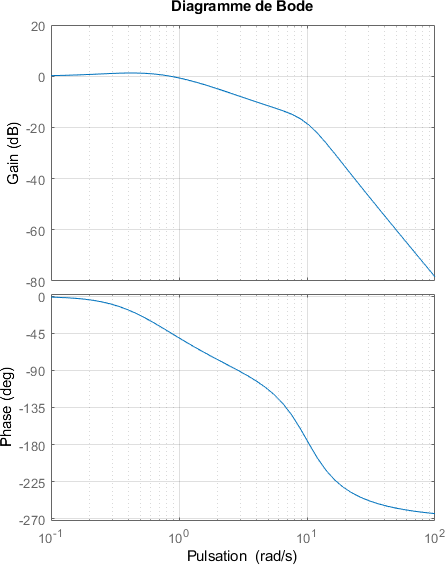
\includegraphics[width=\linewidth]{Q06.png}
%\textit{Cahier des charges de la boucle de régulation de glissement pour $V_T = \SI{200}{km.h^{-1}}$}
\end{center}
\fi


\ifprof
\begin{corrige}
\end{corrige}
\else
\fi


\question{Proposer les valeurs numériques pour les différents paramètres associés à
cette fonction de transfert.}
\ifprof
\begin{corrige}
\begin{itemize}
\item $K_f=1$ : lorsque $\omega$ tend vers 0, le gain tend vers 0;
\item $\omega_0  = 0,5$ : valeur de la pulsation de résonance; 
\item $\tau_1 = \dfrac{1}{0,9}=\SI{1,11}{s}$;
\item $\tau_2 = \dfrac{1}{7} =\SI{0,14}{s}$;
\item $\xi<0,7$ (résonance).
\end{itemize}
\end{corrige}
\else
\fi


\question{En justifiant votre réponse, montrer que l’on peut approcher la fonction de
transfert $F(p)$ par la forme suivante : $ F(p)=\dfrac{\nu_1(p)}{\nu_c(p)}=\dfrac{K_f\left( 1+\tau_1 p\right)}{\left( 1+\tau_2 p\right)^2 } $.}
\ifprof
\begin{corrige}

\begin{center}
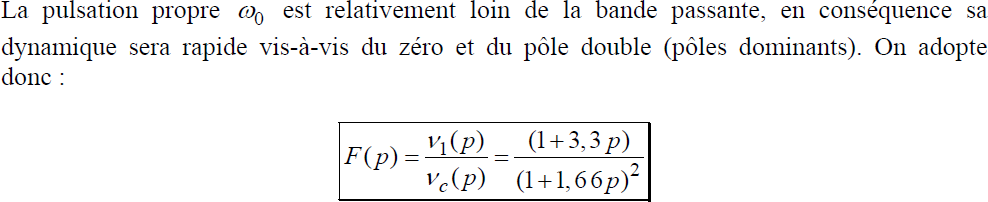
\includegraphics[width=\linewidth]{cor_04.png}
\end{center}
\end{corrige}
\else
\fi

On donne la réponse temporelle vis-à-vis de la consigne de glissement : $f(t)=\left( \dfrac{\tau_2 - \tau_1 }{\tau_2^3 }t +\dfrac{\tau_1}{\tau_2^2} \right)e^{-\dfrac{t}{\tau_2}} u(t)$.




\question{Calculer le temps du 1\ier maximum et en déduire le
dépassement en réponse à une variation en échelon de la consigne de glissement
relatif $\nu_c(t)=\nu_{c0}u(t)$ où $u(t)$ désigne l’échelon unité.}
\ifprof
\begin{corrige}

\begin{center}
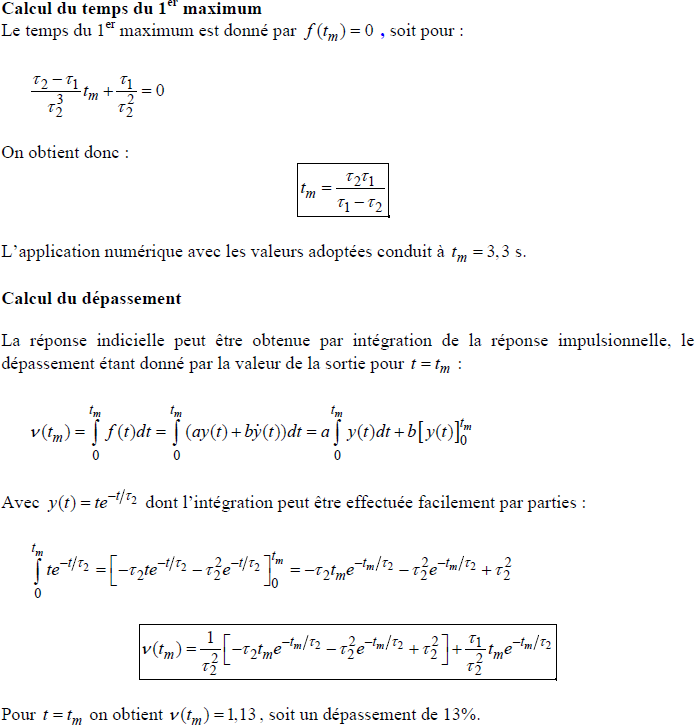
\includegraphics[width=\linewidth]{cor_05.png}
\end{center}
\end{corrige}
\else
\fi


\question{Vérifier le cahier des charges en réponse à une variation en échelon de la consigne de glissement relatif.}
\ifprof
\begin{corrige}
\begin{center}
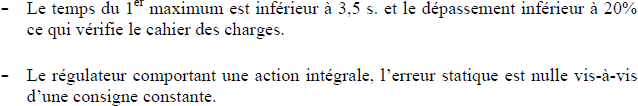
\includegraphics[width=\linewidth]{cor_06.png}
\end{center}
\end{corrige}
\else
\fi

\subsection*{Analyse des performances temporelles en réponse à des variations d’adhérence}
\ifprof
\else
La variation d’adhérence peut être modélisée en première approximation comme une force perturbatrice externe additive . On admet que cette modélisation conduit au schéma bloc représenté sur la figure ci-dessous.

\begin{center}
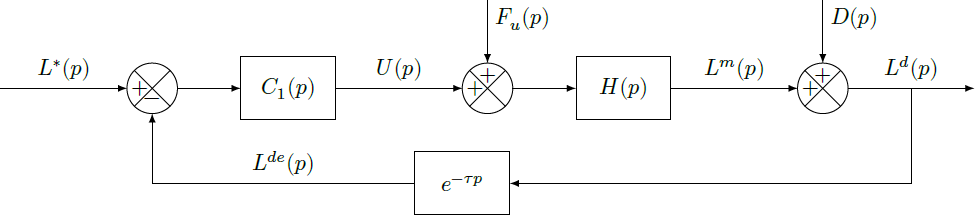
\includegraphics[width=\linewidth]{fig_03}
%\textit{}
\end{center}

On se propose dans cette partie d’évaluer les performances de la chaîne de régulation de freinage vis-à-vis de cette perturbation.

\fi

\question{Déterminer la fonction de transfert $F_2(p)=\dfrac{\nu_1(p)}{F_{\text{ext}}(p)}$ entre le glissement
et la force de perturbation que vous expliciterez en fonction des différentes
transmittances de la boucle de régulation (on suppose $\nu_c$ nulle). En expliquant soigneusement
votre démarche, montrer que le module de la réponse fréquentielle, notée $||F_2(j \omega)||$, de cette fonction peut être approché par la relation :
$||F_2(j \omega)|| = \min \left[ ||H_2(j \omega) || ; \dfrac{1}{||C(j\omega) H_1(j \omega) M(j\omega)||}\right]$ }.

\ifprof
\begin{corrige}
On a directement $F_2(p)=-\dfrac{H_2(p)}{1+H_2(p)M(p)C(p)H_1(p)}$.

On peut alors déterminer le module et on a $||F_2(j\omega)||=\left|\left|\dfrac{H_2(j\omega)}{1+H_2(j\omega)M(j\omega)C(j\omega)H_1(j\omega)}\right|\right|$. 

Dans ces conditions: 
\begin{itemize} 
\item si $\left|\left|{H_2(j\omega)M(j\omega)C(j\omega)H_1(j\omega)}\right|\right|>>1$ alors  $||F_2(j\omega)||\simeq \left|\left|\dfrac{H_2(j\omega)}{H_2(j\omega)M(j\omega)C(j\omega)H_1(j\omega)}\right|\right|\simeq \left|\left|\dfrac{1}{M(j\omega)C(j\omega)H_1(j\omega)}\right|\right|$;
\item si $\left|\left|{H_2(j\omega)M(j\omega)C(j\omega)H_1(j\omega)}\right|\right|<<1$ alors  $||F_2(j\omega)||\simeq \left|\left|{H_2(j\omega)}\right|\right|$.
\end{itemize}

On peut en conclure que $||F_2(j \omega)|| = \min \left[ ||H_2(j \omega) || ; \dfrac{1}{||C(j\omega) H_1(j \omega) M(j\omega)||}\right]$.
\end{corrige}
\else
\fi


% Calcul de la fonction de transfert F_2(p).


\question{La figure suivante comporte le tracé de la fonction $\dfrac{1}{||C(j\omega) H_1(j \omega) M(j\omega)||}$. Tracer
directement sur cette figure le diagramme asymptotique de la fonction $||H_2(j \omega) ||$.}
\ifprof
\else
\begin{center}
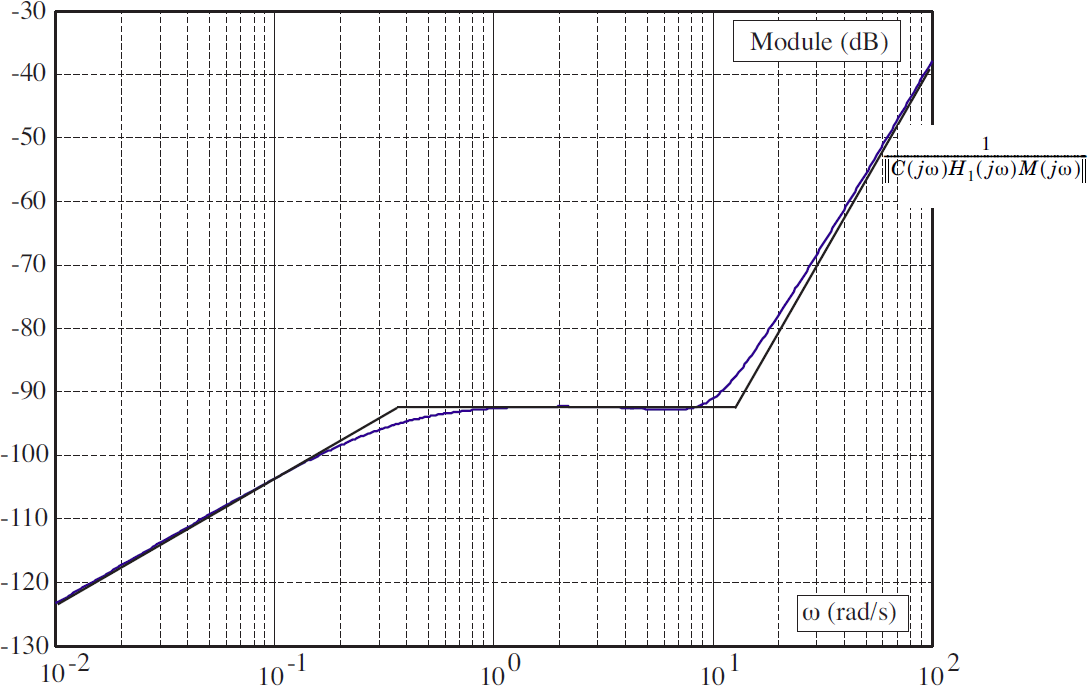
\includegraphics[width=\linewidth]{Q12}
\end{center}
\fi

\ifprof
\begin{corrige}
\begin{center}
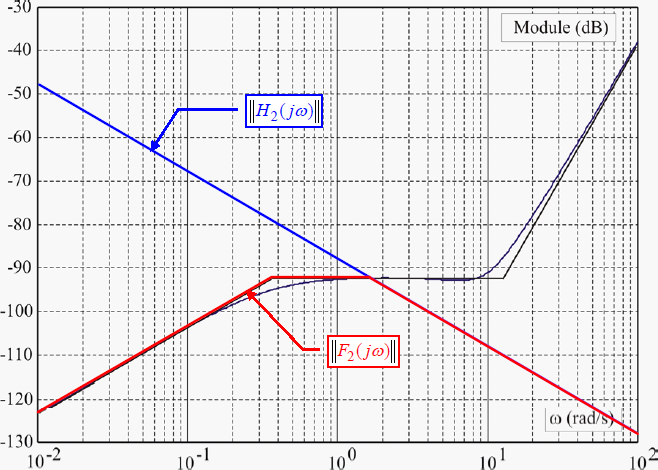
\includegraphics[width=\linewidth]{cor_07.png}
\end{center}
\end{corrige}
\else
\fi



\question{En déduire la forme du tracé asymptotique de la fonction $||F_2(j \omega) ||$. En analysant
les brisures de ce diagramme et en supposant que le système bouclé est
stable, donner directement sous forme numérique, l’expression de la fonction de
transfert $F_2(p)$ entre le glissement et la perturbation due à la
variation d’adhérence.}
\ifprof
\begin{corrige} ~\\
\begin{center}
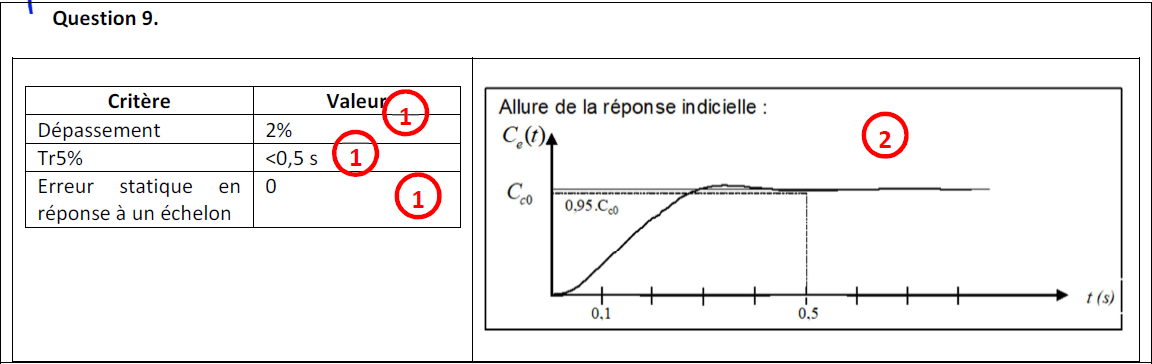
\includegraphics[width=\linewidth]{cor_03}
\end{center}

En analysant les brisures de $F_2$, on peut proposer la fonction de transfert suivante : 
$F_2 = -\dfrac{Kp}{\left(1+\tau_1 p\right)\left(1+\tau_2 p\right)}$ avec $\tau_1 = \dfrac{1}{0,35}\simeq \SI{2,9}{s}$, $\tau_2 = \dfrac{1}{1,8}\simeq \SI{0,6}{s}$. Avec cette proposition, en basse fréquence, seul le dérivateur existe, ona donc  $20 \log K\omega =20\log  0,01K = -123$ soit $K = 100\times 10 ^{-123/20}\simeq 7 \cdot 10^{-5}$. 

Au final, $F_2 = -\dfrac{7 \cdot 10^{-5}p}{\left(1+2,9 p\right)\left(1+0,6 p\right)}$.
\end{corrige}
\else
\fi

%  Calcul de l’évolution du glissement en réponse à une variation de l’adhérence.


\question{Préciser les pôles de la fonction $F_2(p)$ déterminée à la question précédente et en justifiant votre réponse proposer une fonction approchée de cette fonction sous
la forme : $F_2(p)=\dfrac{K_2p}{1+Tp}$.}
\ifprof
\begin{corrige} ~\\

\begin{center}
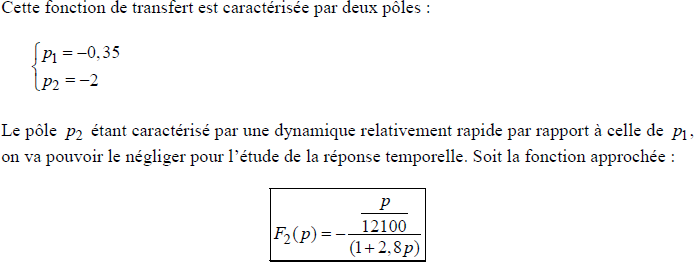
\includegraphics[width=\linewidth]{cor_10}
\end{center}

\end{corrige}
\else
\fi


\question{En utilisant cette fonction de transfert, donner l’expression de l’évolution
temporelle du glissement relatif  $\nu_1(t)$ en réponse à une variation en échelon de
la force perturbatrice $F_{\text{ext}}=F_0u(t)$ , où $u(t)$ représente l’échelon unité et avec
$F_0=\SI{2000}{N}$.}
\ifprof
\begin{corrige}

\begin{center}
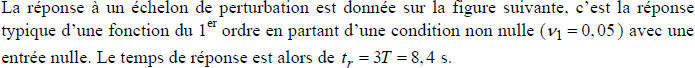
\includegraphics[width=\linewidth]{cor_12}
\end{center}

\end{corrige}
\else
\fi

\question{Tracer l’allure de l’évolution temporelle du glissement relatif $\nu_1(t)$ en précisant
la valeur initiale $\nu_1(0)$. En vous référant à des fonctions ou des résultats
connus, déterminer un ordre de grandeur du temps de réponse $t_r$ à partir
duquel le glissement reste en dessous de 5\,\% de la valeur initiale $\nu_1(0)$ (valeurs
à considérer en valeur absolue).}
\ifprof
\begin{corrige}
\begin{center}
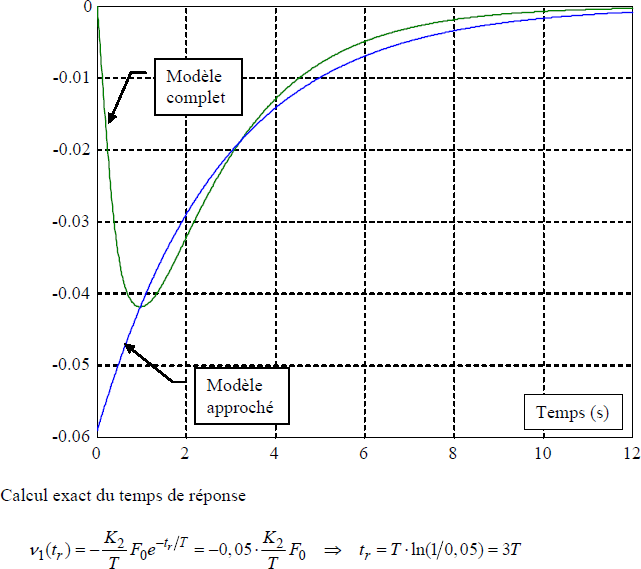
\includegraphics[width=\linewidth]{cor_13}
\end{center}
\end{corrige}
\else
\fi

\subsection*{Retour sur le cahier des charges}

\question{Conclure sur les performances obtenues vis-à-vis des exigences du cahier des charges en réponse à des variations de l’adhérence.}
\ifprof
\begin{corrige}
\begin{center}
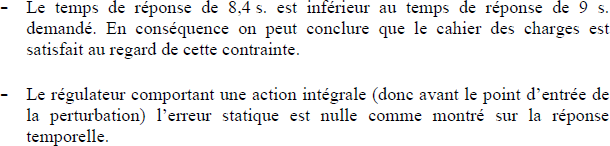
\includegraphics[width=.8\linewidth]{cor_14}
\end{center}
\end{corrige}
\else
\fi

\footnotesize
\begin{enumerate}
\item ...
\item $\arg \left[  \dfrac{T_i p+1}{T_i p}  \right] \geq - \SI{21,5}{\degres}$.
\item $T_i \geq \tan(68,5)=\SI{2,54}{s}$.
\item ***
\item ***
\item ***
\item ***
\item ***
\item ***
\item ***
\end{enumerate}
\normalsize


\ifprof
\else
\end{multicols}
\fi

